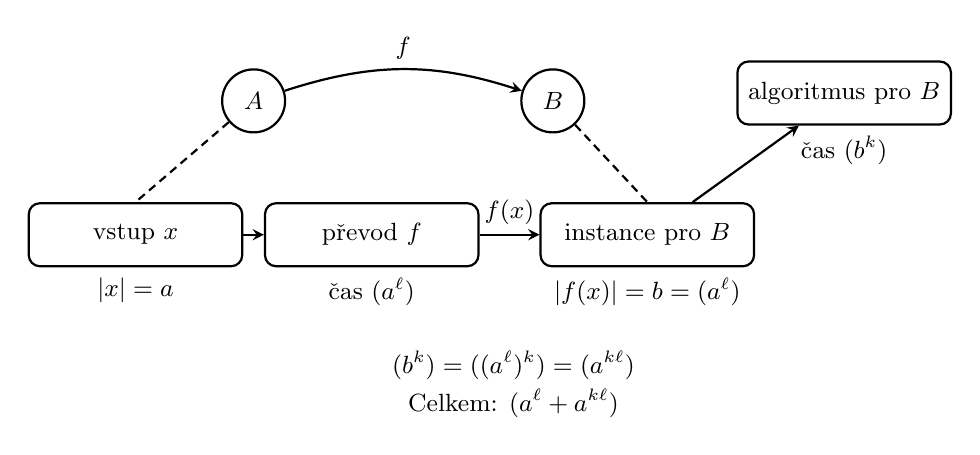
\begin{tikzpicture}[
    >=stealth,
    thick,
    font=\small,
    prob/.style={
        draw,
        circle,
        thick,
        minimum size=8mm,
        inner sep=0pt
    },
    box/.style={
        draw,
        rounded corners,
        thick,
        align=center,
        inner sep=3pt,
        text width=2.5cm,
        minimum height=8mm
    }
]
    % Abstraktni rovina
    \node[prob] (A) at (1.5,0.9) {$A$};
    \node[prob] (B) at (5.3,0.9) {$B$};

    \draw[->, bend left=18]
        (A) to node[midway, above] {$f$} (B);

    % Konkretni vypocet
    \node[box] (x)   at (0.0,-0.8) {vstup $x$};
    \node[box] (red) at (3.0,-0.8) {převod $f$};
    \node[box] (fx)  at (6.5,-0.8) {instance pro $B$};
    \node[box] (alg) at (9.0,+1.0) {algoritmus pro $B$};

    \draw[->] (x) -- (red);
    \draw[->] (red) -- node[midway, above] {$f(x)$} (fx);
    \draw[->] (fx) -- (alg);

    % Propojeni abstraktni a konkretni roviny
    \draw[densely dashed] (A) -- (x.north);
    \draw[densely dashed] (B) -- (fx.north);

    % Popisky slozitosti
    \node[below] at (x.south) {$|x|=a$};
    \node[below] at (red.south) {čas $\bigO(a^\ell)$};
    \node[below] at (fx.south) {$|f(x)|=b=\bigO(a^\ell)$};
    \node[below] at (alg.south) {čas $\bigO(b^k)$};

    % Zaverecny odhad
    \node[align=center] at (4.8,-2.7)
        {$\bigO(b^k)=\bigO((a^\ell)^k)=\bigO(a^{k\ell})$\\[1mm]
         Celkem: $\bigO(a^\ell+a^{k\ell})$};
\end{tikzpicture}